The given equation can be writen as:
\begin{align}
    x^2+1&=3x
\implies     x^2-3x+1&=0 \label{quadform/43/a/eq:2}
    \\
\text{or }\vec{x}^T\myvec{1&0\\0&0}\vec{x}+\myvec{-3&-1}\vec{x}+1&=0
\end{align}
\begin{align}
\because \vec{V} = \myvec{1 & 0 \\ 0 & 0},\vec{u}=\myvec{\frac{-3}{2} \\ \frac{-1}{2}}, f=1,
\end{align}
and
\begin{align}
\vec{D} = \myvec{0 & 0\\0 & 1} ,\vec{P}=\myvec{0 & 1\\1 & 0},
\end{align}

\begin{align}
\myvec{\vec{u}^T + \eta\vec{p_1}^T \\ \vec{V}}\vec{c} &= \myvec{-f \\ \eta\vec{p_1}-\vec{u}} 
\\
\implies \myvec{\frac{-3}{2} & -1 \\ 1 & 0 \\ 0 & 0}\vec{c} &= \myvec{-1\\ \frac{-3}{2} \\ 0} \\
\implies  \myvec{-\frac{-3}{2} & -1 \\ 1 & 0}\vec{c} &= \myvec{-1\\ \frac{3}{2}}
\\
\implies \vec{c} &= \myvec{\frac{3}{2}\\\frac{-5}{4}}
\end{align}
Now,
\begin{align}
\vec{p_1}^T\vec{c} &= \myvec{0 & 1}\myvec{\frac{3}{2}\\\frac{-5}{4}}
\\
&= \frac{-5}{4}
\end{align}
and,
\begin{align}
\vec{p_2}^T\vec{V}\vec{p_2} &= \myvec{1 & 0}\myvec{1 & 0\\0& 0}\myvec{1 \\ 0}
\\
&= 1
\end{align}
$\because$
\begin{align}
(\vec{p_1}^T\vec{c})(\vec{p_2}^T\vec{V}\vec{p_2}) = \frac{-5}{4}<0,
\end{align}
the given equation has real and distinct roots given by 
\begin{align}
\vec{x}&= \myvec{\pm \frac{-2\vec{u^Te_1} \pm \sqrt{(2\vec{u^Te_1})^2-(4\vec{e^T_1Ve_1f})^2}}{2\vec{e^T_1Ve_1}} \\ 0}
\\
&=\myvec{2.6180\\0},\myvec{0.38196\\0}
\end{align}
This is verified in Fig. \ref{quadform/43/a/fig:curve}.	
%
\begin{figure}[!ht]
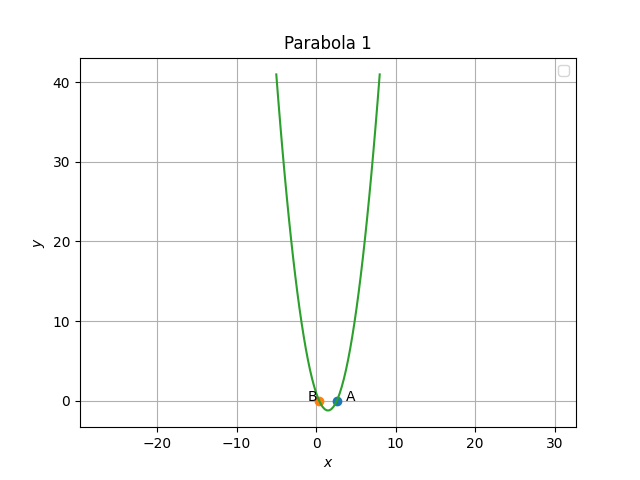
\includegraphics[ width=\columnwidth]{solutions/su2021/2/43/a/Figure/figure.png}
\caption{curve}
\label{quadform/43/a/fig:curve}	
\end{figure}

